\documentclass[12pt]{article}
\usepackage{graphicx}
\usepackage{times}
\usepackage{cite}
\usepackage[utf8]{inputenc}
\usepackage{subfig}
\usepackage{caption}
%this is a comment
\title{The Memo}
\author{Jesse Chick\\
\and Benjamin Martin\\
\and Keenan Johnson\\
\and Nickoli Londura\\
\and Jiaji Sun}




\begin{document}
\maketitle
\tableofcontents

\section{Contributors and ONIDs}
\par
LINK TO THE GITHUB REPO AT THE CORRECT BRANCH: https://github.com/Tonyenike/CS361-001-W2018/tree/the\_memo-assignment-5/projects/martinb3/assignment-5

\begin{itemize}
	\item Jesse Chick $\sim$ chickj
	\item Benjamin Martin $\sim$ martinb3
	\item Keenan Johnson $\sim$ johnsoke
	\item Nickoli Londura $\sim$ londuran
	\item Jiaji Sun $\sim$ sunji
\end{itemize}

\section{User Stories}

\begin{enumerate}
	\item \textbf{View Tutorials.} User may click on a tutorial link to view a tutorial, or a procedure on how to solve a Rubik’s Cube blindfolded.
	\item \textbf{Rotate Cube} User may click on an array to rotate the entire cube in its corresponding direction.
	\item \textbf{Scramble Cube} User may click a scramble button on the cube page to scramble the squares on the cube in such a way that it is still solvable blindfolded.
	\item \textbf{Switch Page} The user may click on a button on the menu sidebar to switch the page that they are currently on.
	\item \textbf{Generate Letters} The user can input a string of random letters, but only letters, and the webpage will generate a string of words for the user to memorize.
	\item \textbf{Check solution} The user can input a solution on the cube page (which will come in the form of a string of letters for move operations), and the webpage will either verify their proposed solution or correct their response.
	\item \textbf{Reset Cube} The user can press a button to reset the cube to solution form (normal, solved, as if it was just bought out of the box).
	\item \textbf{Main Page Redirect} The user may click on the header/title bar to redirect back to the main page, which is the tutorials page on the website.
	\item \textbf{Clear input bar} Upon clicking any input text bar, either on the cube page or the letters page, any text that was previously in the text bar is cleared so that the user can enter a new string.
	\item \textbf{404 Content} Any content that the user requests that doesn’t exist will be served with a 404 page and sent a 404 error to the client.
\end{enumerate}
	
\section{Corresponding Tasks}

\begin{enumerate}
	\item \textbf{View tutorials - 2/28.} This is going to involve embedding the urls from the selected tutorials in the HTML of the tutorials page.
	\item \textbf{Rotate Cube - 3/6 (All cube operations should can be completed in any order unless otherwise noted).} User may click on an array to rotate the entire cube in its corresponding direction.
This will involve calling a member function of the Cube class which will reorient the square values according to how the squares will appear in our visual.

	\item \textbf{Scramble Cube - 3/6.} User may click a scramble button on the cube page to scramble the squares on the cube in such a way that it is still solvable blindfolded. This will require that we adapt a third party algorithm for generating this sort of scramble to our project. This can be done without too much difficulty and we will not forget to cite the source of the algorithm. These values for the cube will be read into the Cube class and its squares set.

	\item \textbf{Switch Page - 3/3.} This is going to involve serving new content via javascript if the user clicks on the respective page’s button in the menu.
	\item \textbf{Generate Letters - 3/3 (Do after Switch Page).} This will likely require the use of a library which contains a batch of common words which span many different permutations of letters. Then, some cost function will be devised to select the best word to fit the letters. This will be a heuristic, but we should be able to make it a very good one. This will be part of the javascript implementation of the page.
	\item \textbf{Check solution - 3/3 (Do after Clear Input Bar).} The user can input a solution on the cube page (which will come in the form of a string of letters for move operations), and the webpage will either verify their proposed solution or correct their response. The correct solution is generated along with the scramble, so the user’s entry into the input bar is compared to the solution using a substring function. The user will then be informed of the validity of their guess based on whether it is a match. Hardcode solutions for testing.

	\item \textbf{Reset Cube - 3/6.} The standard solved layout (significant because it shows the starting layout of the letters) can easily be stored in a data structure, which will overwrite all existing square values.
	\item \textbf{Main Page Redirect - 2/28.} This will involve serving the homepage again in the event that the user clicks on the large header bar atop our application.
	\item \textbf{Clear input bar - 2/28.} Upon clicking any input text bar, either on the cube page or the letters page, any text that was previously in the text bar is cleared so that the user can enter a new string.
	\item \textbf{404 Content - 2/28 (Do first).} This will require event handling to serve this page if an unknown url is entered, etc. 
\end{enumerate}

\section{UML Sequence Diagram/Spike}

\subsection{404 Diagram}
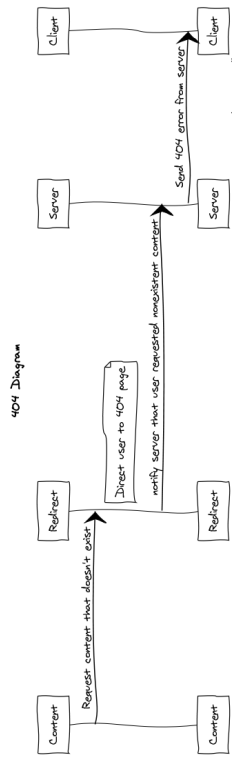
\includegraphics[width = \textwidth]{dia404.PNG}

\subsection{Tutorial Diagram}
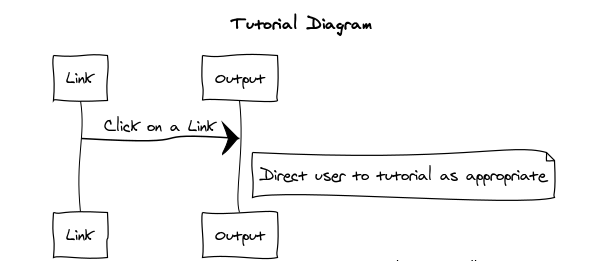
\includegraphics[width = \textwidth]{tut.PNG}

\subsection{Main Page Redirect Diagram}
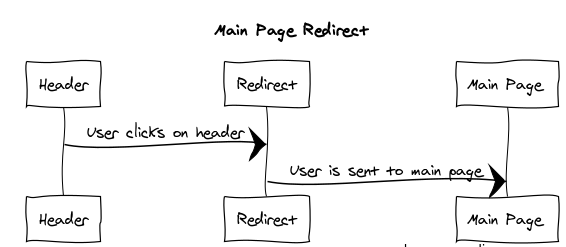
\includegraphics[width = .8\textwidth]{mainpagedia.PNG}

\subsection{Input Bar Diagram}
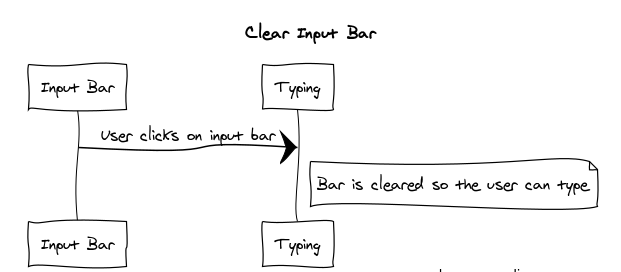
\includegraphics[width = \textwidth]{inputdia.PNG}

\section{The Stories Due Next Week}

\par
The goal for next week is to finish implementing the main framework of our web application. We have already created semi-working prototypes that we can very easily build upon to make a more fleshed out and functional website. \\

\par
We’ll aim to create a barebones page for each function. These would include: tutorials, 404, cube, generate letters, and check solution. Once we have these pages created, we can start working on navigation. We will implement the Switch Page and Main Page Redirect stories. \\

\par
As soon as navigation of these pages has been completed, we can move on to implementing the actual functionality. The View Tutorials story as well as the Generate Letters/Clear Input Bar stories will be the first pages to implement. For View Tutorials, we will just need to populate the page with other resources related to actually learning the methods of blindfolded solving itself. \\

\par
The Generate Letters story is next to be implemented. This will be a matter of creating an input for a pair of letters and then pulling from a predetermined (already have) source of possible words corresponding to the given letter pair and displaying those possibilities. This would also be the ideal point to implement the Clear Input Bar story as we will be using it here for the first time. \\

\section{Meeting Report}

\par
This week is week seven. We haven’t met until this week since we don’t have the assignment in week six. But we keep in touch with every group members. On this week we have met 4 times on campus. Including three times in library and one meeting after class. \\

\par
On our first meeting on Wednesday. We met everyone in the library. Including our customer. The requirement of our customer is not changing. In addition, he very satisfies our project design and our prototype, so we decided not change our design and process plan. First of all, we separate our third phase of the project to every group member. Benjamin Martin is working on user stories and UML sequence diagram/spike. Jiaji Sun is working on meeting report. Jesse Chick is working on corresponding tasks, and Keenan Johnson is working on the stories due next week as well as compiling the algorithms that will be controlling the scramble and solution generation. On this meeting, we have to decide the user stories first, because this part is the most important part of this assignment. Other parts of this assignment depend on user stories. Therefore, we have discussed some most possibility stories that we can imagine. We have tried to imagine all user stories as much as possible. We finally found seven stories at the end. At the end of this meeting, we decided try keep find user stories as much as possible. \\

\par
 On our second meeting, we met after class. Everyone describes new user stories of each other and briefly discussed other parts of this assignment. In the end, we decided ten user stories for our project at the end. \\
 
 \par
 On our third meeting, we keep met in the library. In this meeting, we were working on corresponding tasks. In this meeting, our customer showing up with us. He helped us to find out corresponding tasks as much as possible. In the beginning, We have discussed twenty different corresponding tasks. However, Jesse thought there were ten are not fit for the requirement. Therefore, we decided to delete ten corresponding tasks.  After one hour discussed, we finally settle down ten corresponding tasks. \\
 
 \par
 After the third meeting we only have one section left, so we were working on UML sequence diagram/spike on the fourth meeting. Since our customer is very satisfied our project design and our prototype, we settled our UML sequence diagram/spike very quickly. Therefore, we finished this section very quickly. \\
 
 \par
 In this week, we have met our customer and he helps us to find corresponding tasks. Every group member is working well. They finished their section very nicely. Our plan for next will keep working on implement every function of each module. Try to finish it and test it as soon as possible. \\



\end{document}
